\documentclass[11pt,a4paper]{article}

\usepackage[utf8]{inputenc}
\usepackage[T1]{fontenc}
\usepackage{lmodern}
\usepackage[margin=2.6cm]{geometry}
\usepackage{microtype}
\usepackage{amsmath,amssymb,amsthm,mathtools}
\usepackage{booktabs}
\usepackage{xcolor}
\usepackage{enumitem}
\usepackage{caption}
\usepackage{tikz}
\usepackage{pgfplots}
\usepgfplotslibrary{fillbetween}
\pgfplotsset{compat=1.18}
\usepackage[round,sort&compress]{natbib}
\usepackage[colorlinks=true,linkcolor=blue!50!black,citecolor=blue!50!black,urlcolor=blue!50!black]{hyperref}
\usepackage[capitalise,noabbrev]{cleveref}
\hypersetup{
  pdftitle={Cubic Smoothing Splines on a Uniform Hermite Grid: A Continuous Hodrick-Prescott Filter for Irregular, Weighted Data with Linear-Time Bayesian Inference},
  pdfauthor={Gerben van Veenendaal},
  pdfkeywords={smoothing spline, Hodrick-Prescott filter, Whittaker smoother, Hermite finite elements, Bayesian credible bands},
}
\usepackage{tcolorbox}

% Generated by python/experiments.py -- do not edit.
\newcommand{\numFitLambda}{\ensuremath{0.00977}}
\newcommand{\numFitKnots}{\ensuremath{902}}
\newcommand{\numFitEdf}{\ensuremath{27.9}}
\newcommand{\numFitN}{\ensuremath{77}}
\newcommand{\numFitCoverage}{\ensuremath{97}}
\newcommand{\numExactError}{\ensuremath{6.3\times 10^{-10}}}
\newcommand{\numConvergenceOrder}{\ensuremath{3.2}}
\newcommand{\numConvergenceAtEight}{\ensuremath{2.5\times 10^{-7}}}
\newcommand{\numScaleError}{\ensuremath{4.8\times 10^{-11}}}
\newcommand{\numKernelError}{\ensuremath{6.2\times 10^{-5}}}
\newcommand{\numEquivalentBandwidth}{\ensuremath{1.58}}
\newcommand{\numCutoffYears}{\ensuremath{9.9}}
\newcommand{\numRuFourMonth}{\ensuremath{5.5\times 10^{-4}}}
\newcommand{\numRuFourYear}{\ensuremath{3.3\times 10^{-3}}}
\newcommand{\numRuTwoMonth}{\ensuremath{4.6\times 10^{-2}}}
\newcommand{\numRuTwoYear}{\ensuremath{7.3\times 10^{-2}}}
\newcommand{\numOurMonth}{\ensuremath{4.7\times 10^{-4}}}
\newcommand{\numOurYear}{\ensuremath{2.1\times 10^{-3}}}
\newcommand{\numOurVsHp}{\ensuremath{1.4\times 10^{-4}}}
\newcommand{\numSignalRange}{\ensuremath{1.78}}
\newcommand{\numIwpError}{\ensuremath{3.0\times 10^{-17}}}
\newcommand{\numBridgeError}{\ensuremath{2.0\times 10^{-11}}}
\newcommand{\numCoverage}{\ensuremath{96.0}}
\newcommand{\numGcvBest}{\ensuremath{0.021}}
\newcommand{\numJsMillion}{\ensuremath{303}}
\newcommand{\numPyMillion}{\ensuremath{384}}


\newtheorem{theorem}{Theorem}
\newtheorem{proposition}[theorem]{Proposition}
\newtheorem{lemma}[theorem]{Lemma}
\newtheorem{corollary}[theorem]{Corollary}
\theoremstyle{definition}
\newtheorem{definition}[theorem]{Definition}
\theoremstyle{remark}
\newtheorem{remark}[theorem]{Remark}

\DeclareMathOperator*{\argmin}{arg\,min}
\DeclareMathOperator{\tr}{tr}
\newcommand{\R}{\mathbb{R}}
\newcommand{\E}{\mathbb{E}}
\newcommand{\N}{\mathcal{N}}
\newcommand{\vth}{\boldsymbol{\theta}}
\newcommand{\vphi}{\boldsymbol{\phi}}
\newcommand{\vb}{\mathbf{b}}
\newcommand{\mA}{\mathbf{A}}
\newcommand{\mK}{\mathbf{K}}
\newcommand{\mU}{\mathbf{U}}
\newcommand{\Sd}{\mathcal{S}_\Delta}
\newcommand{\dd}{\,\mathrm{d}}

\definecolor{c1}{HTML}{E0700B}
\definecolor{c2}{HTML}{2F6FB3}
\definecolor{c3}{HTML}{2F8F5B}
\definecolor{c4}{HTML}{8E44AD}

\title{Cubic Smoothing Splines on a Uniform Hermite Grid:\\
A Continuous Hodrick--Prescott Filter for Irregular, Weighted Data\\
with Linear-Time Bayesian Inference}

\author{Gerben van Veenendaal\\\texttt{gerbenvv@gmail.com}}

\date{September 2026}

\begin{document}

\maketitle

\begin{abstract}
The Hodrick--Prescott (HP) filter, and the Whittaker--Henderson graduation it rediscovers, smooths a series by penalizing squared second differences. It requires equally spaced observations, cannot weight them, returns values only at the sampling points, and has a smoothing parameter whose meaning changes with the sampling frequency. We study the continuous counterpart: the penalized least-squares problem $\sum_i w_i\,(y_i-f(x_i))^2+\alpha\int f''(x)^2\dd x$, solved over $C^1$ piecewise cubic Hermite functions on a uniform knot grid chosen independently of the data. The roughness penalty is integrated exactly, giving the Euler--Bernoulli beam element stiffness matrix, and the normal equations form a symmetric positive definite system with seven diagonals, solved in $O(n+m)$ time for $n$ observations and $m$ knots. Writing the smoothing parameter as $\alpha=h^4/L$ turns $h$ into a bandwidth in the units of $x$: the estimator is exactly invariant to rescaling the $x$-axis, acts as a low-pass filter with gain $1/(1+(h\omega)^4)$, and has Silverman's equivalent kernel with bandwidth $h$. The HP filter is the finite-difference discretization of the same functional with $\lambda_{\mathrm{HP}}=(h/\Delta)^4$, which derives the Ravn--Uhlig rule that $\lambda_{\mathrm{HP}}$ must scale with the fourth power of the sampling frequency. We show that the method reproduces the exact cubic smoothing spline whenever the data lie on the grid and converges to it otherwise; that its prior is the exact finite-dimensional marginal of the integrated Wiener process; and that pointwise Gaussian credible bands, posterior samples, effective degrees of freedom and generalized cross-validation all follow in $O(n+m)$ via banded Cholesky factorization and Takahashi selected inversion. We review the extensive related literature and assess candidly which parts are new.
\end{abstract}

\tableofcontents

\section{Introduction}
\label{sec:introduction}

Given a time series $y_1,\dots,y_n$, the Hodrick--Prescott filter \citep{HodrickPrescott1997} computes a trend $\tau$ as
\begin{equation}
\label{eq:hp}
\boldsymbol{\tau}^*=\argmin_{\boldsymbol{\tau}}\;\sum_{i=1}^{n}(y_i-\tau_i)^2+\lambda_{\mathrm{HP}}\sum_{i=2}^{n-1}\bigl(\tau_{i+1}-2\tau_i+\tau_{i-1}\bigr)^2 .
\end{equation}
The idea of penalizing differences of the fitted sequence goes back a century to the actuarial graduation of \citet{Whittaker1922} (who used third differences) and \citet{Henderson1924}, and the second-difference penalty of \eqref{eq:hp} was proposed by \citet{Leser1961} for trend estimation; in chemometrics it is known as the Whittaker smoother \citep{Eilers2003}. It is a discrete analog of the cubic smoothing spline of \citet{Schoenberg1964} and \citet{Reinsch1967}, a relation made precise by \citet{PaigeTrindade2010} and exploited for continuous-time, irregularly sampled versions of the filter by \citet{IannacconeOtranto2003} and \citet{McElroyTrimbur2007}, and it has well-known statistical limitations as a business-cycle tool \citep{Hamilton2018,PhillipsShi2021}.

From a numerical point of view, \eqref{eq:hp} has four limitations:
\begin{enumerate}[label=(\roman*)]
\item it requires equally spaced observations;
\item it cannot weight observations, for example by their measurement precision;
\item its output is a sequence of values at the sampling points, not a function;
\item the meaning of $\lambda_{\mathrm{HP}}$ depends on the sampling frequency: \citet{RavnUhlig2002} showed that $\lambda_{\mathrm{HP}}$ should be multiplied by the fourth power of the ratio of observation frequencies, e.g.\ $1600$ for quarterly data becomes $1600/4^4=6.25$ for annual and $1600\cdot 3^4=129\,600$ for monthly data.
\end{enumerate}

\paragraph{This paper.} We study the continuous problem
\begin{equation}
\label{eq:objective}
f^*=\argmin_{f}\;J(f),\qquad J(f)=\sum_{i=1}^{n}w_i\,\bigl(y_i-f(x_i)\bigr)^2+\frac{h^4}{L}\int_{t_1}^{t_m}f''(x)^2\dd x ,
\end{equation}
for arbitrary locations $x_i$ and weights $w_i\ge 0$ with $\sum_i w_i=1$, where $L$ is a fixed length (by default the length of the domain $[t_1,t_m]$) and $h>0$ is a bandwidth measured in the units of $x$. We minimize over $C^1$ piecewise cubic Hermite functions on a uniform knot grid $t_1<\dots<t_m$ that is chosen independently of the data and may be as fine as desired. This is a penalized regression spline in the sense of \citet{OSullivan1986} and \citet{EilersMarx1996}, and equivalently a Galerkin finite-element discretization of the smoothing-spline variational problem using cubic Hermite elements. The unknowns are the value and the derivative of $f$ at every knot.

\paragraph{Contributions.} The paper collects, proves and verifies the following properties (\cref{sec:novelty} discusses which are new).
\begin{enumerate}[label=\arabic*.]
\item A closed-form discretization: data enter through rank-one $4\times 4$ blocks, the roughness penalty through the beam element stiffness matrix, and the normal equations are symmetric positive definite with half-bandwidth $3$, solved in $O(n+m)$ (\cref{sec:discretization}).
\item Exactness and convergence: if every $x_i$ is a knot the method returns the exact cubic smoothing spline; in general it is the best approximation of that spline in the energy norm of $J$ and converges to it as $\Delta\to 0$ (\cref{sec:exactness}).
\item The bandwidth parametrization $\alpha=h^4/L$: exact scale invariance, transfer function $1/(1+(h\omega)^4)$, Silverman's equivalent kernel with bandwidth $h$ (\cref{sec:bandwidth}).
\item The relation to HP: $\lambda_{\mathrm{HP}}=(h/\Delta)^4$, which derives the Ravn--Uhlig fourth-power rule and gives the HP filter a sampling-independent continuous definition (\cref{sec:hp}).
\item A Bayesian formulation whose prior is the exact integrated-Wiener-process marginal at the knots, with pointwise Gaussian credible bands, posterior sampling, effective degrees of freedom and GCV, all in $O(n+m)$ (\cref{sec:bayes}).
\end{enumerate}

\section{Background}
\label{sec:background}

\paragraph{Graduation and the HP filter.} Whittaker--Henderson graduation \citep{Whittaker1922,Henderson1924} penalizes the $d$-th differences of the fitted sequence; $d=2$ gives \eqref{eq:hp}. It remains an active topic in actuarial science \citep{NoconScott2012,Biessy2025}, where \citet{Biessy2025} gives it a modern Bayesian/REML treatment with credible intervals, and in the physical sciences, where weighted variants handle uneven sampling, derivatives and error bars \citep{Eilers2003,Garcia2010,MulderLagendijkVos2026}. \citet{HodrickPrescott1997} popularized the filter in macroeconomics with $\lambda_{\mathrm{HP}}=1600$ for quarterly data; the same penalty appears earlier in \citet{Leser1961}. Efficient $O(n)$ solvers exploit the pentadiagonal structure \citep{Weinert2007}, closed-form expressions for the filter and its weights exist \citep{CorneaMadeira2017,YamadaJahra2019}, and the smoothing parameter can be estimated by maximum likelihood in a state-space formulation \citep{Schlicht2005}. The filter's model-based interpretation as the optimal extractor of a smooth integrated random walk from noise \citep{KingRebelo1993,HarveyJaeger1993,KaiserMaravall2001}, its frequency response and its dependence on the sampling interval \citep{BaxterKing1999,RavnUhlig2002}, its end-point behavior \citep{MiseKimNewbold2005}, one-sided versions \citep{StockWatson1999} and its econometric properties \citep{deJongSakarya2016} are well studied. Band-pass and model-based alternatives include \citet{BaxterKing1999}, \citet{ChristianoFitzgerald2003}, \citet{Pollock2000}, \citet{Gomez2001} and \citet{HarveyTrimbur2003}; criticism and remedies include \citet{Hamilton2018}, \citet{Hodrick2020} and the boosted HP filter of \citet{PhillipsShi2021}; generalizations handle missing observations \citep{Yamada2020,Yamada2022}. Replacing the squared penalty by an $\ell_1$ penalty gives trend filtering \citep{KimKohBoydGorinevsky2009,Tibshirani2014}, which also accommodates unevenly spaced inputs.

\paragraph{Continuous-time HP filters.} The HP filter is the discrete-time version of the cubic smoothing spline, and continuous-time and irregular-sampling versions have been proposed through this link. \citet{IannacconeOtranto2003} and \citet{OtrantoIannaccone2005} define a generalized HP filter in continuous time for irregularly spaced surveys using the cubic-spline state-space model, and \citet{McElroyTrimbur2007} derive continuous-lag HP and Butterworth filters with irregular spacing and changes of sampling frequency as explicit motivation. State-space software has long offered the continuous-time cubic-spline model \citep{KoopmanShephardDoornik1999,Harvey1989,DurbinKoopman2012}, and observation weights for such signal extraction are discussed by \citet{KoopmanHarvey2003}. \citet{PaigeTrindade2010} proved formally that HP is a penalized spline for equally spaced data.

\paragraph{Cubic smoothing splines.} \citet{Schoenberg1964} and \citet{Reinsch1967} showed that the minimizer of \eqref{eq:objective} over the Sobolev space $W^{2,2}$ is a natural cubic spline with knots at the distinct data locations, computable in $O(n)$ \citep{Reinsch1967,HutchinsonDeHoog1985,DeHoogHutchinson1987,Weinert2009}. Standard references are \citet{Wahba1990}, \citet{GreenSilverman1994}, \citet{Eubank1999}, \citet{deBoor1978}, \citet{Dierckx1993} and, for functional data, \citet{RamsaySilverman2005}. The smoothing parameter is commonly chosen by generalized cross-validation \citep{CravenWahba1979,Silverman1984cv} or marginal likelihood \citep{Wahba1985,Wood2011}. \citet{Silverman1984} showed that the smoothing spline is asymptotically a kernel smoother whose bandwidth is the fourth root of the ratio of the smoothing parameter to the local data density; see also \citet{Silverman1985} and \citet{Nychka1995}.

\paragraph{Penalized regression splines.} Using fewer basis functions than data points, with a roughness penalty, gives penalized regression splines: \citet{OSullivan1986} used cubic B-splines with the exact integrated squared second derivative, \citet{EilersMarx1996,EilersMarx2010} replaced the penalty by differences of B-spline coefficients on equally spaced knots (P-splines), \citet{Wood2017ps} gave exact banded derivative penalties for uniform-knot B-splines applied to unevenly distributed data, and \citet{Ruppert2002} showed that beyond a modest number of knots the fit barely depends on it. \citet{RuppertWandCarroll2003}, \citet{Wand2003}, \citet{WandOrmerod2008} and \citet{Wood2003,Wood2017} developed the methodology into a general framework; \citet{Wood2017} also describes a cubic regression spline parametrized by its knot values. Asymptotic theory, including the many-knot regime in which penalized splines behave like smoothing splines, is due to \citet{HallOpsomer2005}, \citet{LiRuppert2008} and \citet{ClaeskensKrivobokovaOpsomer2009}. Bayesian versions include \citet{LangBrezger2004} and \citet{SpeckmanSun2003}. \citet{CostaShaw2009} parametrize cubic splines by knot values and first derivatives, the Hermite parametrization used here, and interpret quadratic penalties as Gaussian priors; penalized cubic Hermite regression with knots at the data also appears in \citet{CaoEtAl2021} and \citet{CampagnaCotroneiFazzino2025}.

\paragraph{Bayesian and state-space views.} \citet{KimeldorfWahba1970} and \citet{Wahba1978} showed that the smoothing spline is the posterior mean under an integrated Wiener process prior with diffuse initial conditions; \citet{Wahba1983} and \citet{Nychka1988} derived and analyzed the resulting Bayesian confidence intervals, and \citet{AnsleyKohn1986} related the two stochastic formulations. \citet{WeckerAnsley1983} and \citet{KohnAnsley1987} computed the spline in $O(n)$ with the Kalman filter using the value and derivative of $f$ as the state, building on the continuous-time state-space treatment of \citet{Jones1981}; posterior sampling in such models uses simulation smoothers \citep{CarterKohn1994,DurbinKoopman2002}, and \citet{Robinson2010} applies the augmented-state integrated Wiener process to irregular sequential data. Smoothness priors for time series are surveyed by \citet{KitagawaGersch1996}. The modern counterpart is state-space Gaussian-process regression \citep{HartikainenSarkka2010,SarkkaSolinHartikainen2013,SarkkaSolin2019,SolinSarkka2020}; see \citet{RasmussenWilliams2006} for the Gaussian-process view of splines.

\paragraph{Gaussian Markov random fields.} The integrated Wiener process at irregular locations with augmented state $(f,f')$ is a Gaussian Markov random field with block-tridiagonal precision \citep{RueHeld2005,LindgrenRue2008}; \citet{Rue2001} gives fast sampling for such models. \citet{LindgrenRue2008} derive second-order random walks on irregular grids by a Galerkin argument with piecewise-linear elements and explicitly mention, and set aside, the alternative of regular locations combined with interpolation. These models underlie INLA \citep{RueMartinoChopin2009} and the SPDE approach \citep{LindgrenRueLindstrom2011,LindgrenBolinRue2022}, including adaptive smoothing splines \citep{YueSimpsonLindgrenRue2014}. Closest to the present work, \citet{ZhangStringerBrownStafford2024} approximate integrated Wiener processes of any order with finite elements (``overlapping splines'') on a data-independent grid, recommending as many equally spaced knots as computationally feasible, with approximate Bayesian inference \citep{StringerBrownStafford2023}.

\paragraph{Finite elements for smoothing.} Discretizing the smoothing variational problem with finite elements on a grid independent of the data is standard in higher dimensions: \citet{HeglandMcIntoshTurlach1999} fit additive models this way in $O(n)$, \citet{RobertsHeglandAltas2003} analyze the convergence of thin-plate spline approximations with piecewise polynomials, and \citet{Ramsay2002} and \citet{SangalliRamsayRamsay2013} develop spatial spline regression on irregular domains. Two-dimensional Hermite finite elements with a curvature penalty are used to smooth and differentiate displacement fields in digital image correlation \citep{ZhaoEtAl2012,ZhaoSongWu2015}. The cubic Hermite element is the classical element for fourth-order problems such as Euler--Bernoulli beams \citep{Przemieniecki1968,StrangFix1973,Hughes2000,ZienkiewiczTaylorZhu2013}; indeed the spline was named after the draftsman's elastic strip, and \eqref{eq:objective} is the energy of an elastic beam tied to the data by springs of stiffness $w_i$. Banded Cholesky factorization is standard \citep{GolubVanLoan2013}; selected inversion goes back to \citet{TakahashiFaganChin1973} and \citet{ErismanTinney1975}, see \citet{LinEtAl2009} for a modern account.

\section{The estimator}
\label{sec:estimator}

\subsection{Function space}

Let $t_j=t_1+(j-1)\Delta$, $j=1,\dots,m$, be a uniform grid with spacing $\Delta=(t_m-t_1)/(m-1)$ and $t_1\le x_i\le t_m$ for all $i$. Let $\Sd$ be the space of functions on $[t_1,t_m]$ that are cubic polynomials on every interval $[t_j,t_{j+1}]$ and continuously differentiable. A function $f\in\Sd$ is determined by its knot values $f_j=f(t_j)$ and knot derivatives $f'_j=f'(t_j)$, so $\dim\Sd=2m$. $\Sd$ contains the $C^2$ cubic splines on the grid (dimension $m+2$) and is dense in $W^{2,2}[t_1,t_m]$ as $\Delta\to 0$.

\subsection{Cubic Hermite basis}

For $x\in[t_j,t_{j+1}]$ let $z=(x-t_j)/\Delta\in[0,1]$. Then
\begin{equation}
\label{eq:hermite}
f(x)=f_j\,H_0(z)+\Delta f'_j\,H_1(z)+f_{j+1}\,H_2(z)+\Delta f'_{j+1}\,H_3(z),
\end{equation}
with the cubic Hermite basis
\begin{equation}
H_0=(1-z)^2(1+2z),\quad H_1=z(1-z)^2,\quad H_2=z^2(3-2z),\quad H_3=-z^2(1-z).
\end{equation}
An equivalent form is
\begin{equation}
\label{eq:ab-form}
\begin{gathered}
f(x)=(1-z)f_j+z f_{j+1}+z(1-z)\bigl(a_j(1-z)+b_j z\bigr),\\
a_j=\Delta f'_j-(f_{j+1}-f_j),\qquad b_j=-\Delta f'_{j+1}+(f_{j+1}-f_j):
\end{gathered}
\end{equation}
linear interpolation plus a cubic bump that vanishes at both knots.

We collect the parameters, with derivatives scaled by $\Delta$, in
\begin{equation}
\vth=\bigl(f_1,\;\Delta f'_1,\;f_2,\;\Delta f'_2,\;\dots,\;f_m,\;\Delta f'_m\bigr)^\top\in\R^{2m}.
\end{equation}
The scaling makes all parameters carry the units of $y$, which improves conditioning and makes $\vth$ invariant to the scale of the $x$-axis (\cref{thm:scale}). For a point $x$ in element $j$ we write $f(x)=\vphi(x)^\top\vth$, where $\vphi(x)\in\R^{2m}$ is zero except for $\bigl(H_0(z),H_1(z),H_2(z),H_3(z)\bigr)$ in positions $2j-1,\dots,2j+2$. Derivatives follow from $f^{(\nu)}(x)=\Delta^{-\nu}\,\vphi^{(\nu)}(z)^\top\vth$. Locating the element of $x$ is $j=\lfloor (x-t_1)/\Delta\rfloor+1$, so evaluation costs $O(1)$ without any search.

\begin{figure}[t]
\centering
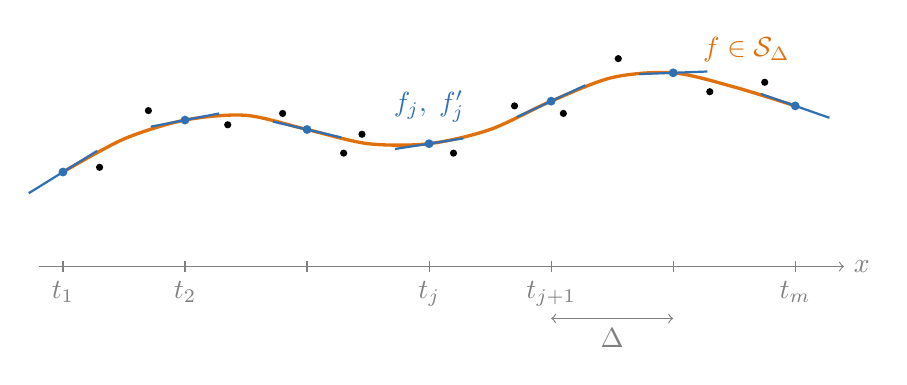
\begin{tikzpicture}[x=1.55cm,y=1.2cm]
\draw[->,gray] (-0.2,0) -- (6.4,0) node[right] {$x$};
\foreach \j in {0,...,6} {
  \draw[gray] (\j,-0.06) -- (\j,0.06);
}
\node[below,gray] at (0,-0.05) {$t_1$};
\node[below,gray] at (1,-0.05) {$t_2$};
\node[below,gray] at (3,-0.05) {$t_j$};
\node[below,gray] at (4,-0.05) {$t_{j+1}$};
\node[below,gray] at (6,-0.05) {$t_m$};
\draw[<->,gray] (4,-0.55) -- node[below] {$\Delta$} (5,-0.55);
\draw[c1,very thick,smooth] plot coordinates {(0,1.0) (0.5,1.35) (1,1.55) (1.5,1.6) (2,1.45) (2.5,1.3) (3,1.3) (3.5,1.45) (4,1.75) (4.5,2.0) (5,2.05) (5.5,1.9) (6,1.7)};
\foreach \x/\y/\s in {0/1.0/0.8, 1/1.55/0.25, 2/1.45/-0.3, 3/1.3/0.2, 4/1.75/0.6, 5/2.05/0.05, 6/1.7/-0.45} {
  \fill[c2] (\x,\y) circle (1.6pt);
  \draw[c2,thick] ({\x-0.28},{\y-0.28*\s}) -- ({\x+0.28},{\y+0.28*\s});
}
\foreach \x/\y in {0.3/1.05, 0.7/1.65, 1.35/1.5, 1.8/1.62, 2.3/1.2, 2.45/1.4, 3.2/1.2, 3.7/1.7, 4.1/1.62, 4.55/2.2, 5.3/1.85, 5.75/1.95} {
  \fill[black] (\x,\y) circle (1.3pt);
}
\node[c2,above] at (3,1.42) {$f_j,\;f'_j$};
\node[c1] at (5.6,2.3) {$f\in\Sd$};
\end{tikzpicture}
\caption{The model. A uniform grid of knots, independent of the data (black dots), carries a value and a derivative per knot (blue); between knots $f$ is the cubic Hermite interpolant (orange).}
\label{fig:concept}
\end{figure}

\subsection{Objective and smoothing parameter}

We minimize \eqref{eq:objective} over $\Sd$. It is convenient to write the smoothing parameter as
\begin{equation}
\label{eq:alpha}
\alpha=\frac{h^4}{L},
\end{equation}
so that $J(f)=\sum_i w_i(y_i-f(x_i))^2+\alpha R(f)$ with roughness $R(f)=\int_{t_1}^{t_m}f''^2$. Since the weights sum to one, the data term has units of $y^2$ and $R$ has units $y^2/x^3$, so $\alpha$ must have units $x^3$; with $L$ a length, $h$ is a length. \Cref{sec:bandwidth} shows that $h$ is the equivalent-kernel bandwidth of the smoother, and \cref{sec:hp} that it is the continuous analog of $\lambda_{\mathrm{HP}}^{1/4}$.

\begin{remark}[Choice of $L$]
\label{rem:L}
A natural choice is $L=t_m-t_1$, the length of the domain. With this choice, enlarging the domain beyond the data (for example to extrapolate) lowers $\alpha$ and so changes the fit. Using the data extent $L=\max_i x_i-\min_i x_i$, or a fixed constant, avoids this; all results below hold for any fixed $L$. When the data are spread evenly over $[t_1,t_m]$, $L=t_m-t_1$ makes $h$ asymptotically the equivalent-kernel bandwidth (\cref{prop:kernel}).
\end{remark}

\section{Discretization and linear-time solution}
\label{sec:discretization}

\subsection{Data term}

Since $f(x_i)=\vphi(x_i)^\top\vth$,
\begin{equation}
\sum_i w_i\bigl(y_i-f(x_i)\bigr)^2=\vth^\top\Bigl(\sum_i w_i\,\vphi_i\vphi_i^\top\Bigr)\vth-2\Bigl(\sum_i w_i y_i\vphi_i\Bigr)^\top\vth+\sum_i w_i y_i^2,
\end{equation}
with $\vphi_i=\vphi(x_i)$. Each observation adds a rank-one $4\times 4$ block to the four parameters of its element.

\subsection{Roughness term}

\begin{lemma}[Element stiffness]
\label{lem:stiffness}
On element $j$, with $\vth_j=(f_j,\Delta f'_j,f_{j+1},\Delta f'_{j+1})^\top$ and $a_j,b_j$ as in \eqref{eq:ab-form},
\begin{equation}
\label{eq:stiffness}
\int_{t_j}^{t_{j+1}}f''(x)^2\dd x=\frac{4}{\Delta^3}\bigl(a_j^2-a_jb_j+b_j^2\bigr)=\frac{1}{\Delta^3}\,\vth_j^\top\mK\,\vth_j,
\qquad
\mK=\begin{pmatrix}12&6&-12&6\\6&4&-6&2\\-12&-6&12&-6\\6&2&-6&4\end{pmatrix}.
\end{equation}
\end{lemma}

\begin{proof}
Differentiating \eqref{eq:ab-form} twice in $z$ gives $\frac{\dd^2 f}{\dd z^2}=2\bigl(b_j-2a_j+3(a_j-b_j)z\bigr)$, and $f''(x)=\Delta^{-2}\frac{\dd^2 f}{\dd z^2}$. Substituting $x=t_j+\Delta z$,
\[
\int_{t_j}^{t_{j+1}}f''^2\dd x=\frac{4}{\Delta^3}\int_0^1\bigl(b_j-2a_j+3(a_j-b_j)z\bigr)^2\dd z=\frac{4}{\Delta^3}\bigl(a_j^2-a_jb_j+b_j^2\bigr),
\]
where the last step is direct integration of a quadratic. Writing $a_j,b_j$ in terms of $\vth_j$ and expanding gives $\mK$; equivalently $\mK=\int_0^1\mathbf H''(z)\mathbf H''(z)^\top\dd z$ with $\mathbf H''=(12z-6,\;6z-4,\;6-12z,\;6z-2)^\top$.
\end{proof}

$\mK$ is the stiffness matrix of the Euler--Bernoulli beam element \citep{Hughes2000}; it is positive semidefinite with null space spanned by the constant and linear functions.

\subsection{Normal equations}

Summing both terms, $J(\vth)=\vth^\top\mA\vth-2\vb^\top\vth+\sum_iw_iy_i^2$ with
\begin{equation}
\label{eq:system}
\mA=\sum_{i=1}^{n}w_i\,\vphi_i\vphi_i^\top+\frac{\alpha}{\Delta^3}\sum_{j=1}^{m-1}\mathbf E_j^\top\mK\,\mathbf E_j,\qquad
\vb=\sum_{i=1}^{n}w_iy_i\,\vphi_i,
\end{equation}
where $\mathbf E_j$ selects the four parameters of element $j$. The minimizer solves $\mA\vth=\vb$.

\begin{proposition}[Structure and solvability]
\label{prop:spd}
$\mA$ is symmetric with half-bandwidth $3$ (seven non-zero diagonals). It is positive definite, and the minimizer is unique, if and only if at least two distinct $x_i$ have positive weight.
\end{proposition}

\begin{proof}
Every term in \eqref{eq:system} couples only the four consecutive parameters $2j-1,\dots,2j+2$ of one element, so $\mA_{kl}=0$ for $|k-l|>3$. $\mA$ is positive semidefinite as a sum of such terms. If $\vth^\top\mA\vth=0$ then $R(f)=0$, so $f$ is linear on $[t_1,t_m]$, and $f(x_i)=0$ wherever $w_i>0$. A linear function with two distinct zeros vanishes, and the Hermite parameters of the zero function are zero, so $\vth=0$. Conversely, if all positive-weight $x_i$ coincide, a linear function through zero at that point is a non-zero null vector.
\end{proof}

\begin{tcolorbox}[colback=gray!4,colframe=gray!50,title=Algorithm 1: fitting in $O(n+m)$,fonttitle=\bfseries]
\begin{itemize}[leftmargin=*,itemsep=2pt]
\item For every observation: $j\gets\lfloor(x_i-t_1)/\Delta\rfloor$ (clamped), $z\gets (x_i-t_1)/\Delta-j$; add $w_i\,\mathbf H(z)\mathbf H(z)^\top$ to the $4\times 4$ block of element $j$ in $\mA$ and $w_iy_i\,\mathbf H(z)$ to $\vb$. \hfill $O(n)$
\item For every element: add $(\alpha/\Delta^3)\,\mK$ to its block. \hfill $O(m)$
\item Banded Cholesky factorization $\mA=\mU^\top\mU$ with $\mU$ upper triangular of bandwidth $3$. \hfill $O(m)$
\item Solve $\mU^\top\mathbf c=\vb$, $\mU\vth=\mathbf c$ by banded substitution. \hfill $O(m)$
\item Evaluate $f(x)$ anywhere in $O(1)$ by \eqref{eq:hermite}; beyond $[t_1,t_m]$ continue linearly with the end slopes (the natural-spline extension).
\end{itemize}
Only the upper band ($4\times 2m$ numbers) is stored. The cost is $O(n+m)$ time and $O(n+m)$ memory.
\end{tcolorbox}

\begin{remark}[Conditioning and the choice of $\Delta$]
\label{rem:conditioning}
For evenly spread data the data term contributes $O(\Delta/L)$ per knot and the roughness term $O(h^4/(L\Delta^3))$, so the condition number of $\mA$ grows like $(h/\Delta)^4$. Knots much finer than $h$ therefore cost accuracy as well as time without improving the fit (\cref{sec:experiments} shows that the discretization error is below $10^{-6}$ of the signal range already at $\Delta=h/8$). We use $\Delta=h/8$ by default.
\end{remark}

\section{Exactness and convergence}
\label{sec:exactness}

Let $f^\star$ denote the minimizer of $J$ over all of $W^{2,2}[t_1,t_m]$: by \citet{Schoenberg1964} and \citet{Reinsch1967} it is the natural cubic spline with knots at the distinct $x_i$, extended linearly to $[t_1,t_m]$ (the Reinsch smoothing spline).

\begin{theorem}[Exactness on the grid]
\label{thm:exact}
If every $x_i$ with $w_i>0$ is a knot, the minimizer of $J$ over $\Sd$ equals $f^\star$ on $[t_1,t_m]$.
\end{theorem}

\begin{proof}
$f^\star$ is a cubic polynomial between consecutive data locations and linear outside them, and is $C^2$. Since every data location is a knot, $f^\star$ is a cubic polynomial on every grid element and $C^1$, so $f^\star\in\Sd$. Minimizing over the subset $\Sd\subset W^{2,2}$ that contains the global minimizer returns the global minimizer, which is unique by \cref{prop:spd}.
\end{proof}

In particular, for equally spaced data with knots at the observations the method is the exact cubic smoothing spline, not the HP filter; extra knots between observations do not change the result. For data off the grid the method is a Galerkin approximation:

\begin{proposition}[Best approximation]
\label{prop:galerkin}
Let $\|g\|_J^2=\sum_iw_ig(x_i)^2+\alpha R(g)$. For all $f\in W^{2,2}$, $J(f)=J(f^\star)+\|f-f^\star\|_J^2$. Consequently the minimizer $f_\Delta$ over $\Sd$ is the $\|\cdot\|_J$-orthogonal projection of $f^\star$ onto $\Sd$,
\[
\|f_\Delta-f^\star\|_J=\min_{g\in\Sd}\|g-f^\star\|_J ,
\]
and $f_\Delta\to f^\star$ as $\Delta\to 0$.
\end{proposition}

\begin{proof}
$J$ is quadratic, so $J(f^\star+e)=J(f^\star)+2\,\delta J(f^\star;e)+\|e\|_J^2$, and the first variation $\delta J(f^\star;e)$ vanishes at the minimizer. Minimizing $J$ over $\Sd$ is therefore minimizing $\|g-f^\star\|_J$ over $g\in\Sd$. Convergence follows because the Hermite interpolant $I_\Delta f^\star\in\Sd$ satisfies $\|I_\Delta f^\star-f^\star\|_J\to 0$: $f^\star$ is piecewise cubic, so the interpolation error is confined to the elements containing a data point, where $f^{\star\prime\prime\prime}$ jumps.
\end{proof}

\Cref{sec:experiments} measures the convergence rate: the maximum error decreases roughly like $(\Delta/h)^{\numConvergenceOrder}$.

\section{The bandwidth parametrization}
\label{sec:bandwidth}

\begin{theorem}[Scale invariance]
\label{thm:scale}
Let $f$ minimize $J$ for data $(x_i,y_i,w_i)$, grid $\{t_j\}$, length $L$ and bandwidth $h$. For $s>0$, the minimizer for the rescaled problem $(s x_i,y_i,w_i)$, $\{s t_j\}$, $sL$, $s h$ is $f_s(x)=f(x/s)$. In particular the parameter vector $\vth$ is unchanged: knot values are identical and knot derivatives are divided by $s$.
\end{theorem}

\begin{proof}
Under the rescaling, $\alpha=h^4/L$ becomes $s^4h^4/(sL)=s^3\alpha$. For any $g$ on $[t_1,t_m]$ let $g_s(x)=g(x/s)$ on $[st_1,st_m]$. Then $g_s(sx_i)=g(x_i)$ and
\[
R(g_s)=\int_{st_1}^{st_m}s^{-4}g''(x/s)^2\dd x=s^{-3}R(g),
\]
so $J_s(g_s)=J(g)$. The map $g\mapsto g_s$ is a bijection from $\Sd$ onto $\mathcal S_{s\Delta}$, hence it maps minimizer to minimizer. Finally $(s\Delta)\,f_s'(st_j)=(s\Delta)\,f'(t_j)/s=\Delta f'(t_j)$, so $\vth$ is unchanged.
\end{proof}

The exponent $4$ is thus forced by dimensional analysis: it is the only power of a length that, divided by one length, has the units $x^3$ of the curvature penalty's coefficient. \citet{Silverman1984} arrived at the same fourth root from the asymptotics of smoothing splines. The next proposition shows that $h$ is literally the bandwidth.

\begin{proposition}[Low-pass filter and equivalent kernel]
\label{prop:kernel}
Suppose the data are dense with constant density on a long interval, so that $\sum_iw_ig(x_i)\to\frac1L\int g(x)\dd x$, and take $L$ equal to the length of that interval. Then the minimizer of $J$ satisfies $f+h^4f''''=y$ away from the boundary, i.e.\ in the Fourier domain
\begin{equation}
\label{eq:gain}
\hat f(\omega)=G(\omega)\,\hat y(\omega),\qquad G(\omega)=\frac{1}{1+(h\omega)^4},
\end{equation}
a low-pass filter with gain $\tfrac12$ at $\omega=1/h$ (period $2\pi h$). Equivalently $f=K_h*y$ with Silverman's kernel
\begin{equation}
\label{eq:kernel}
K_h(u)=\frac{1}{2h}\exp\!\Bigl(-\frac{|u|}{\sqrt2\,h}\Bigr)\sin\!\Bigl(\frac{|u|}{\sqrt2\,h}+\frac{\pi}{4}\Bigr).
\end{equation}
With a non-uniform density $\rho$ (normalized to integrate to one over the domain) the local bandwidth is $h\,(L\rho(x))^{-1/4}$.
\end{proposition}

\begin{proof}
In the limit $J(f)=\frac1L\bigl[\int(y-f)^2+h^4\int f''^2\bigr]$. Its Euler--Lagrange equation is $-(y-f)+h^4f''''=0$; Fourier transformation gives \eqref{eq:gain}, and \eqref{eq:kernel} is the inverse Fourier transform of $G$ \citep{Silverman1984}. For density $\rho$ the data term becomes $\int\rho(y-f)^2$ and the equation $f+\frac{h^4}{L\rho}f''''=y$ holds locally, i.e.\ the bandwidth becomes $h(L\rho)^{-1/4}$.
\end{proof}

\section{Relation to the Hodrick--Prescott filter}
\label{sec:hp}

\begin{theorem}[HP as a finite-difference discretization]
\label{thm:hp}
Let the observations be equally spaced with spacing $\Delta$, $x_i=t_1+(i-1)\Delta$, with equal weights $w_i=1/n$ and $L=n\Delta$. Replacing $f''(t_i)$ by the second difference $(f_{i+1}-2f_i+f_{i-1})/\Delta^2$ and the integral by the rectangle rule turns $J$ into $\frac1n$ times the HP objective \eqref{eq:hp} with
\begin{equation}
\label{eq:hp-lambda}
\lambda_{\mathrm{HP}}=\Bigl(\frac{h}{\Delta}\Bigr)^4,\qquad\text{equivalently}\qquad h=\Delta\,\lambda_{\mathrm{HP}}^{1/4}.
\end{equation}
The HP gain $G_{\mathrm{HP}}(\omega)=\bigl[1+4\lambda_{\mathrm{HP}}(1-\cos\omega\Delta)^2\bigr]^{-1}$ agrees with \eqref{eq:gain} to leading order in $\omega\Delta$ exactly when \eqref{eq:hp-lambda} holds.
\end{theorem}

\begin{proof}
With the stated replacements,
\[
J\approx\frac1n\sum_i(y_i-f_i)^2+\frac{h^4}{n\Delta}\sum_i\Delta\,\frac{(f_{i+1}-2f_i+f_{i-1})^2}{\Delta^4}
=\frac1n\Bigl[\sum_i(y_i-f_i)^2+\frac{h^4}{\Delta^4}\sum_i(f_{i+1}-2f_i+f_{i-1})^2\Bigr].
\]
For the gains, $4(1-\cos\omega\Delta)^2=(\omega\Delta)^4\bigl(1+O(\omega^2\Delta^2)\bigr)$, so $G_{\mathrm{HP}}(\omega)=[1+\lambda_{\mathrm{HP}}\Delta^4\omega^4(1+O(\omega^2\Delta^2))]^{-1}$, which matches $[1+h^4\omega^4]^{-1}$ at leading order if and only if $\lambda_{\mathrm{HP}}\Delta^4=h^4$.
\end{proof}

\begin{corollary}[The Ravn--Uhlig rule]
\label{cor:ru}
Fix the bandwidth $h$ in units of time, i.e.\ fix what is meant by ``trend''. Then the HP parameter must depend on the sampling interval as $\lambda_{\mathrm{HP}}(\Delta)=(h/\Delta)^4$. Sampling $r$ times more often multiplies $\lambda_{\mathrm{HP}}$ by $r^4$:
\[
\lambda_{\mathrm{HP}}^{\text{annual}}=\frac{1600}{4^4}=6.25,\qquad
\lambda_{\mathrm{HP}}^{\text{monthly}}=1600\cdot 3^4=129\,600 .
\]
\end{corollary}

\begin{proof}
Immediate from \eqref{eq:hp-lambda}: $\lambda_{\mathrm{HP}}(\Delta/r)/\lambda_{\mathrm{HP}}(\Delta)=r^4$.
\end{proof}

\citet{RavnUhlig2002} obtained the rule from the frequency response of the HP filter, i.e.\ from the second part of \cref{thm:hp}. In the continuous formulation the rule is not an adjustment but a consequence of the parametrization: $J$ does not refer to the sampling interval at all, the fourth power follows from the units of $\int f''^2$ (\cref{thm:scale}), and one value of $h$ applies to any sampling scheme, including irregular and mixed-frequency data. The customary quarterly value $\lambda_{\mathrm{HP}}=1600$ corresponds to $h=1600^{1/4}=6.32$ quarters $=\numEquivalentBandwidth$ years; by \eqref{eq:gain} cycles longer than $2\pi h\approx\numCutoffYears$ years pass into the trend, consistent with the usual interpretation of $\lambda_{\mathrm{HP}}=1600$ as a cut-off near 10 years (the exact HP half-gain period is $2\pi/\arccos(79/80)=39.7$ quarters).

\begin{figure}[t]
\centering
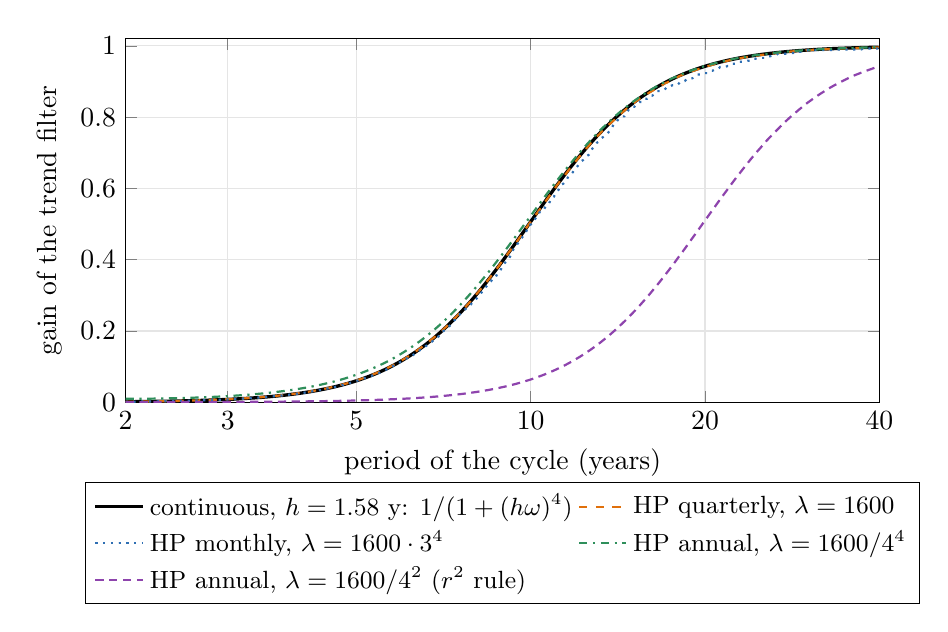
\begin{tikzpicture}
\begin{axis}[
  width=0.92\textwidth, height=6.2cm,
  xmode=log, xmin=2, xmax=40, ymin=0, ymax=1.02,
  xlabel={period of the cycle (years)}, ylabel={gain of the trend filter},
  xtick={2,3,5,10,20,40}, xticklabels={2,3,5,10,20,40},
  legend cell align=left, legend style={font=\small, at={(0.5,-0.22)}, anchor=north, legend columns=2},
  grid=major, grid style={gray!20}, samples=300, domain=2:40,
]
\addplot[black, very thick] {1/(1+(1.5811*2*pi/x)^4)};
\addlegendentry{continuous, $h=1.58$ y: $1/(1+(h\omega)^4)$}
\addplot[c1, thick, dashed] {1/(1+4*1600*(1-cos(deg(2*pi/x*0.25)))^2)};
\addlegendentry{HP quarterly, $\lambda=1600$}
\addplot[c2, thick, dotted] {1/(1+4*129600*(1-cos(deg(2*pi/x/12)))^2)};
\addlegendentry{HP monthly, $\lambda=1600\cdot3^4$}
\addplot[c3, thick, dashdotted] {1/(1+4*6.25*(1-cos(deg(2*pi/x)))^2)};
\addlegendentry{HP annual, $\lambda=1600/4^4$}
\addplot[c4, thick, densely dashed] {1/(1+4*100*(1-cos(deg(2*pi/x)))^2)};
\addlegendentry{HP annual, $\lambda=1600/4^2$ ($r^2$ rule)}
\end{axis}
\end{tikzpicture}
\caption{Frequency response of trend filters. HP filters at three sampling frequencies with $\lambda_{\mathrm{HP}}$ scaled by the fourth power of the frequency ratio (\cref{cor:ru}) all approximate the continuous gain \eqref{eq:gain} with $h=1600^{1/4}$ quarters; scaling by the square instead gives a much smoother annual trend.}
\label{fig:gain}
\end{figure}

\begin{table}[t]
\centering
\caption{Trends from the same noise-free signal (a linear trend plus 30- and 6-year cycles, range $\numSignalRange$) sampled monthly, quarterly and annually for 60 years. Entries are the maximum absolute difference from the quarterly trend at common annual dates, 5 years away from the ends. The continuous method uses one $h=\numEquivalentBandwidth$ years for all samplings.}
\label{tab:ru}
\begin{tabular}{lcc}
\toprule
& monthly vs.\ quarterly & annual vs.\ quarterly\\
\midrule
HP, $\lambda_{\mathrm{HP}}$ scaled by $r^4$ (Ravn--Uhlig) & \numRuFourMonth & \numRuFourYear\\
HP, $\lambda_{\mathrm{HP}}$ scaled by $r^2$ & \numRuTwoMonth & \numRuTwoYear\\
Continuous, fixed $h$ & \numOurMonth & \numOurYear\\
\bottomrule
\end{tabular}
\end{table}

\Cref{fig:gain} and \cref{tab:ru} confirm this. With the $r^4$ rule the HP trends at different sampling frequencies agree to within $\numRuFourYear$, an order of magnitude or more better than with the $r^2$ rule, and the continuous method with a single $h$ matches them, differing from the quarterly HP trend by only $\numOurVsHp$. The remaining differences between samplings are due to the sampling itself (an annual series sees a 6-year cycle with only six points per period), not to the choice of smoothing parameter.

\section{Bayesian formulation and uncertainty}
\label{sec:bayes}

\subsection{Model and posterior}

Assume $y_i=f(x_i)+\varepsilon_i$ with independent $\varepsilon_i\sim\N(0,\sigma_i^2)$. If the $\sigma_i$ are known, set $w_i\propto\sigma_i^{-2}$ and $S=\sum_i\sigma_i^{-2}$. If only relative precisions are known, write $\sigma_i^2=\sigma^2/(nw_i)$ (so $\sigma^2$ is the variance of an observation of average weight) and $S=n/\sigma^2$. In both cases the log-likelihood is $-\tfrac S2\sum_iw_i(y_i-f(x_i))^2$ up to a constant. Take the (partially improper) smoothness prior
\begin{equation}
\label{eq:prior}
p(f)\propto\exp\Bigl(-\frac{S\alpha}{2}\int_{t_1}^{t_m}f''(x)^2\dd x\Bigr),
\end{equation}
which is flat on linear functions. Restricted to $\Sd$, the posterior is $p(\vth\mid\mathbf y)\propto\exp(-\tfrac S2J(\vth))$, i.e.
\begin{equation}
\label{eq:posterior}
\vth\mid\mathbf y\;\sim\;\N\bigl(\mA^{-1}\vb,\;(S\mA)^{-1}\bigr).
\end{equation}
The posterior mean, which is also the mode, is the penalized least-squares fit of \cref{sec:discretization}; the posterior precision is the same banded matrix, scaled by $S$. The prior scale $S\alpha$ depends on the noise level, as in \citet{Wahba1978}, where the smoothing parameter is the ratio of noise to prior variance.

\subsection{The prior is the integrated Wiener process}

\begin{theorem}[Exact marginal]
\label{thm:iwp}
Let $f$ be an integrated Wiener process, $f''=\sqrt{q}\,\dot W$, with diffuse initial state, and let $\mathbf s_j=(f(t_j),f'(t_j))$. The joint density of $\mathbf s_1,\dots,\mathbf s_m$ is proportional to
\[
\exp\Bigl(-\frac{1}{2q}\sum_{j=1}^{m-1}\frac{1}{\Delta^3}\vth_j^\top\mK\vth_j\Bigr),
\]
which is \eqref{eq:prior} evaluated on the Hermite interpolant of the states, with $q=1/(S\alpha)$. Given the states, the conditional mean of $f$ on $[t_j,t_{j+1}]$ is the cubic Hermite interpolant \eqref{eq:hermite}, and the conditional variance at $t_j+s$ is
\begin{equation}
\label{eq:bridge}
q\,\frac{s^3(\Delta-s)^3}{3\Delta^3}\;\le\;\frac{q\Delta^3}{192}.
\end{equation}
\end{theorem}

\begin{proof}
The state $\mathbf s(t)$ is Markov with $\mathbf s_{j+1}=\mathbf F\mathbf s_j+\mathbf e_j$, $\mathbf e_j\sim\N(0,q\mathbf Q)$ \citep{Jones1981,WeckerAnsley1983}, where
\[
\mathbf F=\begin{pmatrix}1&\Delta\\0&1\end{pmatrix},\qquad \mathbf Q=\begin{pmatrix}\Delta^3/3&\Delta^2/2\\\Delta^2/2&\Delta\end{pmatrix}.
\]
Hence $-2q\log p=\sum_j(\mathbf s_{j+1}-\mathbf F\mathbf s_j)^\top\mathbf Q^{-1}(\mathbf s_{j+1}-\mathbf F\mathbf s_j)+\text{const}$. Direct computation shows that $\begin{psmallmatrix}-\mathbf F&\mathbf I\end{psmallmatrix}^\top\mathbf Q^{-1}\begin{psmallmatrix}-\mathbf F&\mathbf I\end{psmallmatrix}=\mathbf D\mK\mathbf D/\Delta^3$ with $\mathbf D=\operatorname{diag}(1,\Delta,1,\Delta)$, which is \cref{lem:stiffness} in the coordinates $(f,f')$. (This is the classical fact that the transition density exponent equals the minimal energy $\int g''^2$ over functions with the given end values and slopes, attained by the cubic Hermite interpolant.) The conditional mean and variance follow from Gaussian conditioning on the four end conditions.
\end{proof}

We verified both identities numerically: the precision matrices agree to $\numIwpError$ (relative) and \eqref{eq:bridge} to $\numBridgeError$. Hence the grid model is the integrated-Wiener-process (Wahba) model with one approximation: an observation between knots sees the conditional mean of $f$ and ignores the bridge variance \eqref{eq:bridge}. When all observations are on knots the posterior \eqref{eq:posterior} is exactly Wahba's Bayesian smoothing spline, the Bayesian counterpart of \cref{thm:exact}. Between knots the bands of the finite-dimensional model are therefore slightly narrower than those of the exact spline posterior; adding the bridge variance \eqref{eq:bridge}, which is at most $q\Delta^3/192$ with $q=1/(S\alpha)$, is a simple conservative correction, negligible for $\Delta\ll h$.

\subsection{A Gaussian distribution at every point}

Because $f(x)=\vphi(x)^\top\vth$ is linear in $\vth$, the posterior at any $x$ is Gaussian:
\begin{equation}
\label{eq:pointwise}
f(x)\mid\mathbf y\;\sim\;\N\Bigl(\vphi(x)^\top\hat\vth,\;\frac1S\,\vphi(x)^\top\mA^{-1}\vphi(x)\Bigr),
\end{equation}
and for the derivatives
\begin{equation}
\label{eq:pointwise-derivative}
f^{(\nu)}(x)\mid\mathbf y\;\sim\;\N\Bigl(\tfrac{\vphi^{(\nu)}(x)^\top\hat\vth}{\Delta^\nu},\;\tfrac{\vphi^{(\nu)}(x)^\top\mA^{-1}\vphi^{(\nu)}(x)}{S\,\Delta^{2\nu}}\Bigr).
\end{equation}
Since $\vphi(x)$ has four consecutive non-zeros, the variance needs only a $4\times 4$ diagonal block of $\mA^{-1}$, which lies within the band. Beyond $[t_1,t_m]$, $\vphi(x)$ is the row of the linear extension, $(1,(x-t_m)/\Delta)$ on the last knot's parameters (and likewise on the first knot's below $t_1$), so the band widens linearly as in \cref{fig:fit}. A pointwise $95\%$ credible band is $\hat f(x)\pm1.96\,\mathrm{sd}(x)$; a predictive band for a new observation adds $\sigma^2$ to the variance. When $\sigma^2$ is estimated, the marginal is approximately a Student-$t$ with $n-\mathrm{edf}$ degrees of freedom, which is indistinguishable from the Gaussian for moderate $n$.

\subsection{Noise level, degrees of freedom and GCV}

The fitted values are $\hat y=\mathbf H\mathbf y$ with hat matrix $\mathbf H=\Phi\mA^{-1}\Phi^\top\mathbf W$, so the effective degrees of freedom are
\begin{equation}
\mathrm{edf}=\tr\mathbf H=\sum_{i=1}^n w_i\,\vphi_i^\top\mA^{-1}\vphi_i ,
\end{equation}
ranging from $2$ (a straight line, $h\to\infty$) to $n$ (interpolation, $h\to 0$, data on knots). The usual estimator of the noise level is
\begin{equation}
\hat\sigma^2=\frac{n\sum_iw_i(y_i-\hat f(x_i))^2}{n-\mathrm{edf}},
\end{equation}
and the generalized cross-validation score \citep{CravenWahba1979} is $\mathrm{GCV}(h)=n\sum_iw_i(y_i-\hat f(x_i))^2/(1-\mathrm{edf}/n)^2$. Both need only the band of $\mA^{-1}$.

\subsection{Linear-time selected inversion and sampling}
\label{sec:selinv}

Given $\mA=\mU^\top\mU$, the Takahashi recursion \citep{TakahashiFaganChin1973,ErismanTinney1975} computes the entries of $\boldsymbol\Sigma=\mA^{-1}$ inside the band from $\mU\boldsymbol\Sigma=\mU^{-\top}$: for $i=2m,\dots,1$ and $j=i+3,\dots,i$,
\begin{equation}
\Sigma_{ij}=\frac{\delta_{ij}}{U_{ii}^2}-\frac{1}{U_{ii}}\sum_{k=i+1}^{i+3}U_{ik}\,\Sigma_{kj},
\end{equation}
which only references already computed entries within the band, at a cost of $O(m)$. The full inverse $\mA^{-1}$ is dense, but it is never formed: every quantity we need (pointwise variances, edf, GCV) is a quadratic form in four consecutive parameters, whose entries lie within distance $3$ of the diagonal. Posterior samples are $\vth=\hat\vth+S^{-1/2}\mU^{-1}\boldsymbol\epsilon$ with $\boldsymbol\epsilon\sim\N(0,\mathbf I)$, one banded back-substitution per sample, because $\operatorname{Cov}(\mU^{-1}\boldsymbol\epsilon)=\mA^{-1}$.

\section{Experiments}
\label{sec:experiments}

All numbers and figures in this section were computed with a direct implementation of \cref{sec:discretization,sec:bayes}.

\paragraph{Irregular, heteroscedastic data.} \Cref{fig:fit} shows $\numFitN$ observations of a known function with a gap and with three times larger noise on the right; weights are the known precisions and $h=\numFitLambda$ was chosen by GCV. The grid has $\numFitKnots$ knots and the fit uses $\numFitEdf$ effective degrees of freedom. The credible band widens in the gap, on the noisy part and beyond the data; it contains the true function on $\numFitCoverage\%$ of the domain. Over 100 replications with GCV-chosen $h$ the average pointwise coverage of the $95\%$ band is $\numCoverage\%$, in line with the across-the-function coverage property of Bayesian spline intervals \citep{Wahba1983,Nychka1988}.

\begin{figure}[t]
\centering
\begin{tikzpicture}
\begin{axis}[
  width=0.95\textwidth, height=7cm, xmin=-0.05, xmax=1.05, ymin=-1.5, ymax=4.5,
  xlabel={$x$}, ylabel={$y$}, legend pos=north west, legend cell align=left, legend style={font=\small},
  grid=major, grid style={gray!15},
]
\addplot[name path=upper, draw=none, forget plot] table[x=x, y expr=\thisrow{f}+1.96*\thisrow{sd}] {data/fit_curve.dat};
\addplot[name path=lower, draw=none, forget plot] table[x=x, y expr=\thisrow{f}-1.96*\thisrow{sd}] {data/fit_curve.dat};
\addplot[c1!22] fill between[of=upper and lower];
\addlegendentry{95\% credible band}
\foreach \c in {s1,s2,s3,s4} {
  \addplot[c1!55, thin, forget plot] table[x=x, y=\c] {data/fit_samples.dat};
}
\addplot[c1, very thick] table[x=x, y=f] {data/fit_curve.dat};
\addlegendentry{posterior mean}
\addplot[black, dashed] table[x=x, y=truth] {data/fit_curve.dat};
\addlegendentry{true function}
\addplot[only marks, mark=*, mark size=1.2pt, black, error bars/.cd, y dir=both, y explicit, error bar style={gray}]
  table[x=x, y=y, y error=sigma] {data/fit_points.dat};
\addlegendentry{data $\pm\sigma_i$}
\end{axis}
\end{tikzpicture}
\caption{Fit to irregular data with a gap ($0.45<x<0.62$) and heteroscedastic noise, with the pointwise $95\%$ credible band \eqref{eq:pointwise} and four posterior samples.}
\label{fig:fit}
\end{figure}

\paragraph{Exactness and convergence.} For 101 equally spaced observations with knots at the observations, and with 2 or 4 knots per observation interval, the maximum difference from SciPy's exact smoothing spline \citep[\texttt{make\_smoothing\_spline}]{Virtanen2020} is $\numExactError$ (\cref{thm:exact}). For 200 irregularly spaced observations, \cref{fig:convergence} shows the maximum error relative to the signal range as a function of $h/\Delta$: it decreases at order about $\numConvergenceOrder$ and is $\numConvergenceAtEight$ at the default $\Delta=h/8$, independently of $h$, as the scale invariance predicts.

\paragraph{Scale invariance and equivalent kernel.} Rescaling $x$ and $h$ by factors from $10^{-6}$ to $10^6$ changes the knot values by at most $\numScaleError$. For dense uniform data the response to a unit impulse matches Silverman's kernel \eqref{eq:kernel} to a relative error of $\numKernelError$ (\cref{fig:kernel}).

\begin{figure}[t]
\centering
\begin{minipage}[t]{0.49\textwidth}
\begin{tikzpicture}
\begin{axis}[
  width=\textwidth, height=6cm, xmode=log, ymode=log,
  xlabel={knots per bandwidth $h/\Delta$}, ylabel={max error / range},
  legend pos=south west, legend style={font=\scriptsize}, grid=major, grid style={gray!15},
]
\addplot[c1, thick, mark=*] table[x=ratio, y=error] {data/convergence_0.01.dat};
\addlegendentry{$h=0.01$}
\addplot[c2, thick, mark=square*] table[x=ratio, y=error] {data/convergence_0.03.dat};
\addlegendentry{$h=0.03$}
\addplot[c3, thick, mark=triangle*] table[x=ratio, y=error] {data/convergence_0.1.dat};
\addlegendentry{$h=0.1$}
\end{axis}
\end{tikzpicture}
\caption{Distance to the exact smoothing spline for irregular data.}
\label{fig:convergence}
\end{minipage}\hfill
\begin{minipage}[t]{0.49\textwidth}
\begin{tikzpicture}
\begin{axis}[
  width=\textwidth, height=6cm, xmin=-6, xmax=6,
  xlabel={$u/h$}, ylabel={$h\,K(u)$},
  legend pos=north east, legend style={font=\scriptsize}, grid=major, grid style={gray!15},
]
\addplot[c1, very thick] table[x=u, y=ours] {data/kernel.dat};
\addlegendentry{impulse response}
\addplot[black, dashed, thick] table[x=u, y=silverman] {data/kernel.dat};
\addlegendentry{Silverman kernel}
\end{axis}
\end{tikzpicture}
\caption{Equivalent kernel for dense uniform data, $h=0.05$.}
\label{fig:kernel}
\end{minipage}
\end{figure}

\paragraph{Smoothing-parameter selection.} \Cref{fig:gcv} shows the GCV score and the effective degrees of freedom as functions of $h$ for 150 noisy observations; the minimum is at $h=\numGcvBest$.

\paragraph{Timing.} \Cref{fig:timing} shows wall-clock times for $n=m$ from $10^3$ to $10^6$ on a laptop. Both implementations scale linearly. With a million observations and a million knots the fit takes $\numJsMillion$\,ms in JavaScript (Node.js) and $\numPyMillion$\,ms in Python (NumPy with LAPACK banded routines through SciPy); the selected inverse, needed for uncertainty, costs a similar amount in JavaScript and more in Python, where it is a pure-Python loop.

\begin{figure}[t]
\centering
\begin{minipage}[t]{0.49\textwidth}
\begin{tikzpicture}
\begin{axis}[
  width=0.86\textwidth, height=6cm, xmode=log,
  xlabel={bandwidth $h$}, ylabel={GCV}, axis y line*=left,
  grid=major, grid style={gray!15}, ymode=log,
]
\addplot[c1, very thick] table[x=lam, y=gcv] {data/gcv.dat}; \label{plot:gcv}
\end{axis}
\begin{axis}[
  width=0.86\textwidth, height=6cm, xmode=log, axis y line*=right, axis x line=none,
  ylabel={edf}, ymode=log,
  legend style={font=\scriptsize, at={(0.5,0.97)}, anchor=north},
]
\addlegendimage{/pgfplots/refstyle=plot:gcv}\addlegendentry{GCV}
\addplot[c2, thick, dashed] table[x=lam, y=edf] {data/gcv.dat};
\addlegendentry{edf}
\end{axis}
\end{tikzpicture}
\caption{GCV score and effective degrees of freedom.}
\label{fig:gcv}
\end{minipage}\hfill
\begin{minipage}[t]{0.49\textwidth}
\begin{tikzpicture}
\begin{axis}[
  width=0.92\textwidth, height=6cm, xmode=log, ymode=log,
  xlabel={$n=m$}, ylabel={time (ms)},
  legend style={font=\scriptsize, at={(0.5,-0.28)}, anchor=north, legend columns=2}, grid=major, grid style={gray!15},
]
\addplot[c1, thick, mark=*] table[x=n, y=js] {data/timing.dat};
\addlegendentry{JavaScript fit}
\addplot[c1, thick, dashed, mark=o] table[x=n, y=jsband] {data/timing.dat};
\addlegendentry{JavaScript selected inverse}
\addplot[c2, thick, mark=square*] table[x=n, y=py] {data/timing.dat};
\addlegendentry{Python fit}
\addplot[c2, thick, dashed, mark=square] table[x=n, y=pyband] {data/timing.dat};
\addlegendentry{Python selected inverse}
\addplot[gray, domain=1000:1000000] {x/3000};
\addlegendentry{linear reference}
\end{axis}
\end{tikzpicture}
\caption{Run time, linear in $n+m$.}
\label{fig:timing}
\end{minipage}
\end{figure}

\section{Related work and novelty}
\label{sec:novelty}

\Cref{tab:comparison} compares the method with the closest existing approaches.

\begin{table}[t]
\centering
\small
\caption{Comparison with related smoothers. ``Grid'': basis independent of the data locations; ``exact $R$'': the integrated squared second derivative rather than a difference approximation. ($\checkmark$): knots are usually placed at quantiles of the data, but may be uniform.}
\label{tab:comparison}
\resizebox{\textwidth}{!}{%
\begin{tabular}{lcccccc}
\toprule
Method & irregular $x$ & weights & function & exact $R$ & grid & cost\\
\midrule
HP / Whittaker \citep{HodrickPrescott1997,Whittaker1922} & -- & -- & -- & -- & -- & $O(n)$\\
Smoothing spline \citep{Reinsch1967} & \checkmark & \checkmark & \checkmark & \checkmark & -- & $O(n)$\\
Kalman spline \citep{WeckerAnsley1983,KohnAnsley1987} & \checkmark & \checkmark & \checkmark & \checkmark & -- & $O(n)$\\
O'Sullivan spline \citep{OSullivan1986,WandOrmerod2008} & \checkmark & \checkmark & \checkmark & \checkmark & ($\checkmark$) & $O(n+m)$\\
P-spline \citep{EilersMarx1996} & \checkmark & \checkmark & \checkmark & -- & \checkmark & $O(n+m)$\\
Continuous-time HP \citep{IannacconeOtranto2003,McElroyTrimbur2007} & \checkmark & \checkmark & \checkmark & \checkmark & -- & $O(n)$\\
Augmented IWP GMRF \citep{RueHeld2005,LindgrenRue2008} & \checkmark & \checkmark & \checkmark & \checkmark & -- & $O(n)$\\
O-splines \citep{ZhangStringerBrownStafford2024} & \checkmark & \checkmark & \checkmark & \checkmark & \checkmark & $O(n+m)$\\
This paper & \checkmark & \checkmark & \checkmark & \checkmark & \checkmark & $O(n+m)$\\
\bottomrule
\end{tabular}}
\end{table}

\paragraph{What is known.} The estimator is a penalized regression spline with the exact roughness penalty, in the sense of \citet{OSullivan1986}; the difference is the basis. O'Sullivan splines use $C^2$ cubic B-splines (dimension $m+2$) and give a banded system with half-bandwidth $3$ as well \citep{WandOrmerod2008,Wood2017ps}, whereas we use $C^1$ cubic Hermite elements (dimension $2m$), i.e.\ the Galerkin finite-element discretization of the smoothing-spline problem. The Hermite parametrization by knot values and derivatives is the state vector of the Kalman-filter smoothing spline \citep{WeckerAnsley1983,KohnAnsley1987} and was used for penalized splines by \citet{CostaShaw2009}; the prior it induces is the augmented-state integrated Wiener process \citep{RueHeld2005,LindgrenRue2008}. Finite-element approximations of the integrated Wiener process on a fine, data-independent, equally spaced grid are the subject of \citet{ZhangStringerBrownStafford2024}, and \citet{LindgrenRue2008} name the regular-grid-plus-interpolant route explicitly. Continuous-time and irregular-sampling HP filters were proposed by \citet{IannacconeOtranto2003}, \citet{OtrantoIannaccone2005} and \citet{McElroyTrimbur2007}. The Bayesian interpretation and credible bands are due to \citet{Wahba1978,Wahba1983}, the equivalent kernel and the fourth-root bandwidth to \citet{Silverman1984}, the $O(m)$ band inverse to \citet{TakahashiFaganChin1973} and \citet{HutchinsonDeHoog1985}, the HP--spline equivalence to \citet{Schoenberg1964}, \citet{KingRebelo1993} and \citet{PaigeTrindade2010}, and the fourth-power rule to \citet{RavnUhlig2002}.

\paragraph{Assessment.} Every component of the method is established, and a continuous-time HP filter for irregular data is not new. We found no single publication with exactly this combination: $C^1$ cubic Hermite elements on a uniform data-independent grid, the exact beam-stiffness penalty, weighted irregular data, a seven-diagonal solve, exact pointwise Gaussian bands in $O(n+m)$, and the $h^4/L$ bandwidth normalization, presented as a direct continuous replacement of the HP filter. Given the prior art above, however, the combination is a small step, and we do not claim a new estimator. What this paper offers is:
\begin{itemize}[itemsep=2pt]
\item the parametrization $\alpha=h^4/L$ with weights normalized to one, which makes the smoothing parameter a sampling-independent length and yields $\lambda_{\mathrm{HP}}=(h/\Delta)^4$, deriving the Ravn--Uhlig rule from the units of the roughness penalty rather than from the filter's frequency response (without normalized weights the identity acquires a factor $n$: $h=\Delta(n\lambda_{\mathrm{HP}})^{1/4}$ for unit weights);
\item a self-contained account of the uniform Hermite grid: exactness when the data lie on the grid (\cref{thm:exact}), the energy-norm projection property otherwise (\cref{prop:galerkin}), the exact integrated-Wiener-process marginal with the bridge variance \eqref{eq:bridge} as the only approximation (\cref{thm:iwp}), and $O(1)$ evaluation;
\item a complete $O(n+m)$ pipeline: fit, exact pointwise Gaussian bands via selected inversion, posterior samples, effective degrees of freedom and GCV.
\end{itemize}

\section{Conclusion}
\label{sec:conclusion}

Minimizing weighted squared error plus $(h^4/L)\int f''^2$ over cubic Hermite functions on a uniform grid gives a smoother that is continuous, accepts irregular and weighted data, has a smoothing parameter measured in the units of $x$, reproduces the exact cubic smoothing spline on the grid, and delivers exact Gaussian posterior uncertainty, all in linear time. Its discrete, equally spaced special case is the Hodrick--Prescott filter with $\lambda_{\mathrm{HP}}=(h/\Delta)^4$, which explains why the HP parameter must scale with the fourth power of the sampling frequency. The method assembles well-established results from spline smoothing, finite elements and Gaussian Markov random fields; its value lies in making them available as one simple, fast and well-understood tool.


\bibliographystyle{plainnat}
\bibliography{references}

\end{document}
